\documentclass[12pt]{article}

% ===== Configuración común =====
\newcommand{\commonpath}{../../common}
% ===== Idioma y codificación =====
\usepackage[spanish, es-nodecimaldot]{babel}
\usepackage[utf8]{inputenc}
\usepackage[T1]{fontenc}
\usepackage{textcomp}

% ===== Tipografía moderna =====
\usepackage{helvet}
\renewcommand{\familydefault}{\sfdefault}
\usepackage{microtype}
\usepackage{xcolor}

% ===== Márgenes y formato =====
\usepackage[a4paper,top=2.8cm,bottom=2.8cm,left=3cm,right=3cm]{geometry}
\usepackage{titlesec}
\titleformat{\section}{\Large\bfseries}{\thesection.\ }{0.4em}{}
\titleformat{\subsection}{\large\bfseries}{\thesubsection.\ }{0.4em}{}
\titlespacing*{\section}{0pt}{1.6ex plus .5ex minus .2ex}{1.0ex}
\titlespacing*{\subsection}{0pt}{1.2ex plus .5ex minus .2ex}{0.7ex}

% ===== Colores =====
\definecolor{UMABlue}{RGB}{0,51,102}

% ===== Paquetes útiles =====
\usepackage{amsmath}
\usepackage{amssymb}
\usepackage{graphicx}
\usepackage{booktabs}
\usepackage{tabularx}
\usepackage{siunitx}
\usepackage{float}
\usepackage{enumitem}
\usepackage{listings}
\usepackage[hidelinks]{hyperref}
\usepackage{tikz}
\usetikzlibrary{arrows.meta, decorations.markings, patterns}
\sisetup{locale=DE}

% ===== Estilo para listados de código =====
\lstset{
  language=C++,
  basicstyle=\ttfamily\footnotesize,
  keywordstyle=\bfseries\color{UMABlue},
  commentstyle=\itshape\color{gray},
  stringstyle=\color{red!60!black},
  numbers=left,
  numberstyle=\tiny\color{gray},
  numbersep=6pt,
  frame=single,
  framerule=0.4pt,
  rulecolor=\color{gray!50},
  breaklines=true,
  tabsize=4,
  showstringspaces=false,
  captionpos=b,
  aboveskip=8pt,
  belowskip=6pt,
}

% ===== Comandos personalizados — Ampliación de Robótica =====

% --- Abreviaturas frecuentes ---
\newcommand{\ros}{ROS~2}
\newcommand{\roshumble}{ROS~2 Humble}
\newcommand{\coppelia}{CoppeliaSim}
\newcommand{\pioneer}{Pioneer P3DX}

% --- Unidades ---
\newcommand{\ms}{\si{\meter\per\second}}
\newcommand{\hz}[1]{\SI{#1}{\hertz}}
\newcommand{\rad}{\si{\radian}}

% --- Pendiente (texto rojo para secciones por completar) ---
\newcommand{\pendiente}[1]{\textcolor{red}{\textbf{[PENDIENTE:} #1\textbf{]}}}

% ===== Portada reutilizable =====
% Uso: \portada{LAB-ID}{Título}{Subtítulo}
\newcommand{\portada}[3]{%
  {%
    \pagecolor{UMABlue}%
    \color{white}%
    \thispagestyle{empty}%
    \begin{center}
      \vspace*{0.8cm}
      
\includegraphics[width=0.22\textwidth]{\commonpath/img/logo_uma.png}\\[0.5cm]
      {\large UNIVERSIDAD DE MÁLAGA\\[0.3cm]}
      {\small Grado en Ingeniería Electrónica, Robótica y Mecatrónica\\[1.2cm]}
      {\huge\bfseries Memoria de Práctica\\[0.6cm]}
      {\LARGE\bfseries #1\\[0.2cm]}
      {\Large\bfseries #2\\[0.4cm]}
      {\normalsize\itshape #3\\[1.8cm]}
      {\normalsize Ampliación de Robótica\\[0.8cm]}
      {\large
        Saúl Gutiérrez Rodríguez\\[0.15cm]
        Pablo Haro García\\[0.15cm]
        Mario Merino Prado\\[0.8cm]
      }
      \rule{0.55\textwidth}{0.4pt}\\[0.3cm]
      {\small
        Repositorio: \texttt{github.com/marioomerino24/ampliacion\_robotica}\\[0.1cm]
        Entorno: \roshumble{} · \coppelia{} · \pioneer{}
      }
    \end{center}
    \clearpage
  }%
  \nopagecolor%
  \color{black}%
}

\graphicspath{{figures/}{\commonpath/img/}}

% ===== Documento =====
\begin{document}

\portada{Lab-MR1.2}{Seguimiento de trayectorias impl\'{i}citas}%
        {Corridor-following con LiDAR y Pure Pursuit}

\tableofcontents
\clearpage


% =====================================================================
%  1. INTRODUCCIÓN
% =====================================================================
\section{Introducci\'{o}n}

\subsection{Objetivo de la pr\'{a}ctica}
El objetivo es implementar un comportamiento reactivo de \textbf{seguimiento de pasillo} (\emph{corridor-following}) para un robot \pioneer{} con tracci\'{o}n diferencial en \coppelia{}. A diferencia de la pr\'{a}ctica anterior, el robot no dispone de waypoints: la trayectoria est\'{a} definida \textbf{impl\'{i}citamente} por la geometr\'{i}a del pasillo, y el robot debe inferirla a partir de las lecturas de un sensor l\'{a}ser 2D.

\subsection{Descripci\'{o}n del problema}
El robot debe recorrer un pasillo cerrado de anchura conocida $W$, manteniendo su posici\'{o}n centrada entre ambas paredes y negociando curvas cuando el pasillo cambia de direcci\'{o}n. No dispone de mapa previo ni planificador global: la navegaci\'{o}n es puramente reactiva, basada en las distancias medidas por el l\'{a}ser en cada instante.

El problema se descompone en:
\begin{enumerate}[leftmargin=2em]
  \item \textbf{Estimaci\'{o}n del estado}: determinar la posici\'{o}n lateral y la orientaci\'{o}n del robot respecto al eje del pasillo a partir de las lecturas l\'{a}ser.
  \item \textbf{Control de centrado}: aplicar una ley de control que corrija el error lateral y angular.
  \item \textbf{Detecci\'{o}n de curvas}: identificar cu\'{a}ndo el pasillo gira y conmutar a un modo de giro apropiado.
\end{enumerate}


% =====================================================================
%  2. FUNDAMENTOS TEÓRICOS
% =====================================================================
\section{Fundamentos te\'{o}ricos}

\subsection{Modelo cinem\'{a}tico del robot}
El \pioneer{} utiliza tracci\'{o}n diferencial con par\'{a}metros $R = \SI{0.097518}{\meter}$ (radio de rueda) y $2K = \SI{0.331}{\meter}$ (distancia entre ruedas). La cinem\'{a}tica directa es:
\begin{equation}
  v = \frac{(\omega_i + \omega_d)\,R}{2}, \qquad
  \omega = \frac{(\omega_d - \omega_i)\,R}{2K}
  \label{eq:cin_directa}
\end{equation}

En esta pr\'{a}ctica se comanda directamente $(v, \omega)$ al simulador a trav\'{e}s del topic \texttt{cmd\_vel}, por lo que no es necesaria la conversi\'{o}n a velocidades de rueda.

\subsection{Algoritmo de control: Pure Pursuit}
\textbf{Pure Pursuit} es un algoritmo de seguimiento de trayectorias geom\'{e}trico que calcula la curvatura necesaria para que el robot alcance un punto objetivo situado a una distancia de \emph{look-ahead} $L$ por delante.

Dado un punto objetivo con coordenada lateral $y_L$ en el sistema de referencia del robot, la curvatura comandada es:
\begin{equation}
  \kappa = \frac{2\,y_L}{L^2}
  \label{eq:pure_pursuit}
\end{equation}

La velocidad angular resultante se obtiene como $\omega = \kappa \cdot v$ y se satura al l\'{i}mite $\omega_\text{max}$.

En el contexto de seguimiento de pasillo, el punto objetivo no pertenece a una trayectoria expl\'{i}cita sino que se construye a partir del error lateral y la orientaci\'{o}n estimada:
\begin{equation}
  y_L = e_\text{lat} \cdot \cos\theta - L \cdot \sin\theta
  \label{eq:yl}
\end{equation}

donde $e_\text{lat}$ es el error lateral respecto al centro del pasillo y $\theta$ es el \'{a}ngulo de orientaci\'{o}n del robot respecto al eje del mismo.

\subsection{Procesamiento sensorial}
El l\'{a}ser 2D realiza un barrido frontal de $180^\circ$. Para extraer informaci\'{o}n robusta de las lecturas individuales se utiliza una funci\'{o}n de \textbf{promediado en ventana angular} (\texttt{averageRangeInWindow}): dada una direcci\'{o}n central y un semiancho de ventana, se promedian todas las lecturas finitas dentro de ese arco. Las direcciones de inter\'{e}s son:

\begin{itemize}[leftmargin=2em]
  \item \textbf{Laterales} ($\pm 90^\circ$, ventana $\pm 1^\circ$): distancias $d_\text{left}$ y $d_\text{right}$ a las paredes.
  \item \textbf{Frontal} ($0^\circ$, ventana $\pm 5^\circ$): distancia $d_\text{front}$ para seguridad.
  \item \textbf{Anticipaci\'{o}n} ($-45^\circ$, ventana $\pm 5^\circ$): distancia $d_\text{right\_ahead}$ para detecci\'{o}n temprana de curvas.
  \item \textbf{Orientaci\'{o}n} ($\pm 75^\circ$ y $\pm 105^\circ$, ventana $\pm 2^\circ$): para estimar el signo de $\theta$.
\end{itemize}

La orientaci\'{o}n del robot respecto al eje del pasillo se estima geom\'{e}tricamente:
\begin{equation}
  |\theta| = \arccos\!\left(\frac{W}{d_\text{left} + d_\text{right}}\right)
  \label{eq:theta_mag}
\end{equation}

El \textbf{signo} de $\theta$ se determina comparando lecturas a $\pm 15^\circ$ de la pared m\'{a}s cercana: si la lectura ``delantera'' ($75^\circ$ o $-75^\circ$) es menor que la ``trasera'' ($105^\circ$ o $-105^\circ$), el robot apunta hacia esa pared, lo que define el signo.


% =====================================================================
%  3. DISEÑO E IMPLEMENTACIÓN
% =====================================================================
\section{Dise\~{n}o e implementaci\'{o}n}

\subsection{Arquitectura del sistema}
El sistema se compone de un \'{u}nico nodo \ros{} que se comunica con \coppelia{} mediante tres topics. El Cuadro~\ref{tab:nodos} resume la arquitectura.

\begin{table}[H]
  \centering
  \caption{Nodos y topics \ros{} del sistema.}
  \label{tab:nodos}
  \begin{tabularx}{0.98\linewidth}{l l X}
    \toprule
    \textbf{Elemento} & \textbf{Tipo} & \textbf{Funci\'{o}n} \\
    \midrule
    \texttt{corr\_nav\_node}            & Nodo (C++) & Lee l\'{a}ser y odometr\'{i}a, ejecuta Pure Pursuit, publica velocidades. \\
    \texttt{/PioneerP3DX/laser\_scan}  & \texttt{LaserScan}  & Barrido l\'{a}ser 2D (180$^\circ$). \\
    \texttt{/PioneerP3DX/odom}         & \texttt{Odometry}   & Pose y velocidades del robot. \\
    \texttt{/PioneerP3DX/cmd\_vel}     & \texttt{Twist}      & Comandos de velocidad. \\
    \bottomrule
  \end{tabularx}
\end{table}

El bucle de control opera a 40~Hz (\SI{25}{\milli\second}).

\subsection{Estrategia de control}
El nodo implementa dos modos de operaci\'{o}n:

\paragraph{Modo recto (Pure Pursuit).}
Se calcula el error lateral $e_\text{lat} = d_\text{left} - W/2$ y la coordenada del punto de look-ahead $y_L$ seg\'{u}n la ecuaci\'{o}n~\eqref{eq:yl}. La curvatura $\kappa = 2\,y_L / L^2$ se traduce en velocidad angular:
\[
  v = \frac{v_\text{max}}{4} = \SI{0.25}{\meter\per\second}, \qquad
  \omega = \text{clamp}(\kappa \cdot v,\; -\omega_\text{max},\; \omega_\text{max})
\]

\paragraph{Modo curva.}
Se activa cuando alguna lectura lateral o de anticipaci\'{o}n indica la desaparici\'{o}n de la pared derecha:
\[
  d_\text{right} > W \;\lor\; d_\text{right\_ahead} > W \implies \text{modo curva}
\]

En este modo se aplica velocidad lineal reducida y giro m\'{a}ximo a la derecha:
\[
  v = \frac{v_\text{max}}{8} = \SI{0.125}{\meter\per\second}, \qquad
  \omega = -\omega_\text{max} = -\SI{0.79}{\radian\per\second}
\]

La lectura de anticipaci\'{o}n a $-45^\circ$ es clave: al tener componente frontal, detecta la apertura del pasillo \textbf{antes} de que el haz a $-90^\circ$ la perciba.

\subsection{Parametrizaci\'{o}n}
Los par\'{a}metros se cargan desde \texttt{corr\_params.yaml}. El Cuadro~\ref{tab:parametros} recoge los valores finales.

\begin{table}[H]
  \centering
  \caption{Par\'{a}metros del controlador \emph{corridor-following}.}
  \label{tab:parametros}
  \begin{tabularx}{0.98\linewidth}{l l X}
    \toprule
    \textbf{Par\'{a}metro} & \textbf{Valor} & \textbf{Descripci\'{o}n} \\
    \midrule
    \texttt{time\_step}             & \SI{25}{\milli\second} & Periodo del bucle de control (40~Hz). \\
    \texttt{max\_linear\_speed}     & \SI{1.0}{\meter\per\second} & Velocidad lineal m\'{a}xima. \\
    \texttt{max\_angular\_speed}    & \SI{0.79}{\radian\per\second} & Velocidad angular m\'{a}xima ($\approx 45^\circ$/s). \\
    \texttt{wheel\_base} ($2K$)     & \SI{0.331}{\meter} & Distancia entre ruedas. \\
    \texttt{wheel\_radius} ($R$)    & \SI{0.097518}{\meter} & Radio de las ruedas. \\
    \texttt{corridor\_width} ($W$)  & \SI{4.2}{\meter} & Anchura del pasillo. \\
    \texttt{look\_ahead\_distance} ($L$) & \SI{4.0}{\meter} & Distancia de look-ahead. \\
    \bottomrule
  \end{tabularx}
\end{table}


% =====================================================================
%  4. RESULTADOS EXPERIMENTALES
% =====================================================================
\section{Resultados experimentales}

\subsection{Escenarios de prueba}
El controlador se ha evaluado en los mundos de \coppelia{} proporcionados para la pr\'{a}ctica: pasillos rectos y con curvas a la derecha.

\subsection{An\'{a}lisis cuantitativo}

\begin{table}[H]
  \centering
  \caption{Resultados del \emph{corridor-following} en diferentes escenarios.}
  \label{tab:resultados}
  \begin{tabularx}{0.98\linewidth}{l c X}
    \toprule
    \textbf{Escenario} & \textbf{Resultado} & \textbf{Observaci\'{o}n} \\
    \midrule
    Pasillo recto ($W = \SI{4.2}{\meter}$) & $\checkmark$ & Robot centrado, error lateral $< \pm\SI{0.1}{\meter}$. \\
    Pasillo con curva a la derecha & $\checkmark$ & Anticipaci\'{o}n a $-45^\circ$ detecta la curva; giro controlado. \\
    Pasillo con curvas consecutivas & $\checkmark$ & Transici\'{o}n correcta entre modos recto y curva. \\
    \bottomrule
  \end{tabularx}
\end{table}

El Cuadro~\ref{tab:velocidades} resume las velocidades comandadas en cada modo.

\begin{table}[H]
  \centering
  \caption{Velocidades seg\'{u}n el modo de operaci\'{o}n.}
  \label{tab:velocidades}
  \begin{tabularx}{0.85\linewidth}{l c c X}
    \toprule
    \textbf{Modo} & $v$ (\si{\meter\per\second}) & $\omega$ (\si{\radian\per\second}) & \textbf{Criterio de activaci\'{o}n} \\
    \midrule
    Recto (Pure Pursuit) & 0.25 & $\kappa \cdot v$ (saturado) & $d_\text{right} \leq W$ y $d_\text{right\_ahead} \leq W$ \\
    Curva derecha         & 0.125 & $-0.79$ & $d_\text{right} > W$ o $d_\text{right\_ahead} > W$ \\
    \bottomrule
  \end{tabularx}
\end{table}

\subsection{An\'{a}lisis cualitativo}
En los tramos rectos, el robot mantiene una posici\'{o}n estable en torno al centro del pasillo. La velocidad de crucero de \SI{0.25}{\meter\per\second} produce un seguimiento suave sin oscilaciones.

En las curvas a la derecha, la lectura a $-45^\circ$ detecta la apertura del pasillo entre 1 y 2~metros antes de que el robot llegue al punto de giro. El controlador conmuta a modo curva y el robot negocia el giro sin colisionar.

\begin{figure}[H]
  \centering
  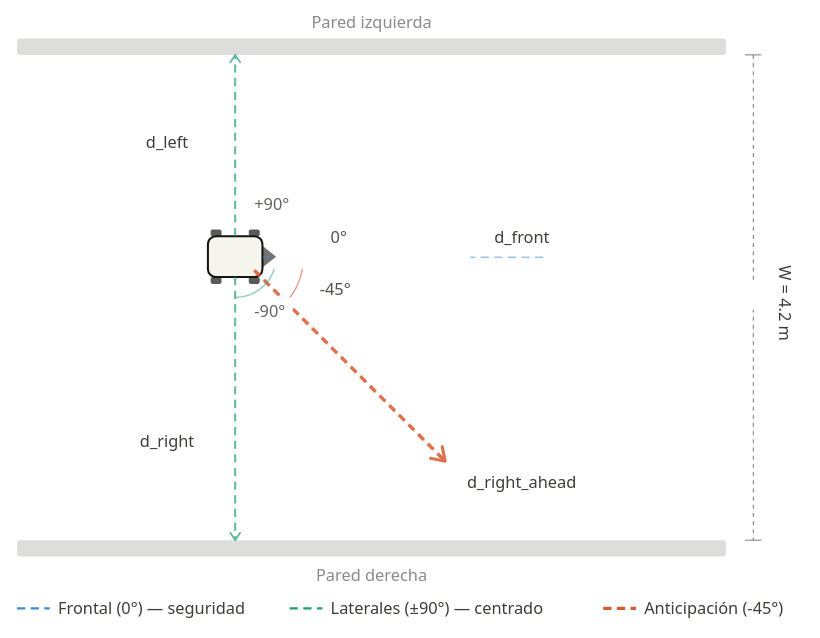
\includegraphics[width=0.55\linewidth]{dibujo_rayos.png}
  \caption{Disposici\'{o}n de los haces l\'{a}ser utilizados: laterales a $\pm 90^\circ$ para el centrado, frontal a $0^\circ$ para seguridad, y anticipaci\'{o}n a $-45^\circ$ para detecci\'{o}n de curvas.}
  \label{fig:angulo}
\end{figure}

\begin{figure}[H]
  \centering
  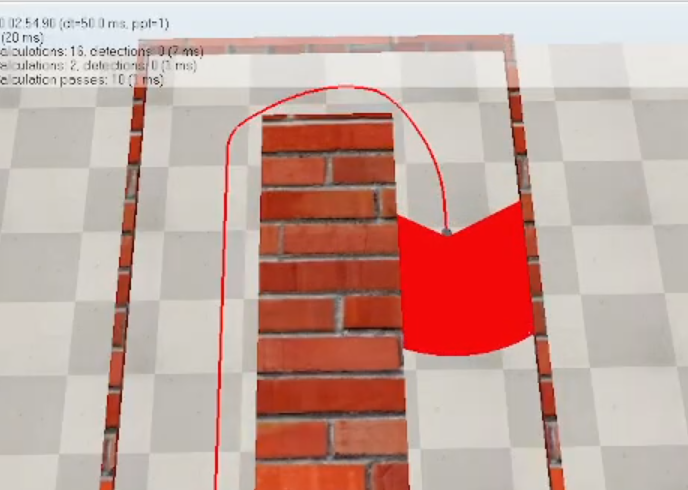
\includegraphics[width=0.75\linewidth]{curvas.png}
  \caption{Robot \pioneer{} navegando por el pasillo en \coppelia{}. Se observa el centrado en el tramo recto y la transici\'{o}n al modo curva.}
  \label{fig:trayectoria}
\end{figure}


% =====================================================================
%  5. DISCUSIÓN
% =====================================================================
\section{Discusi\'{o}n}

\subsection{Problemas encontrados y soluciones}

\paragraph{Problema 1: dependencia de escena en la detecci\'{o}n frontal.}
La primera versi\'{o}n utilizaba la lectura frontal para decidir cu\'{a}ndo girar. El umbral de distancia que funcionaba en un pasillo estrecho provocaba colisiones en pasillos anchos. \textbf{Soluci\'{o}n}: se sustituy\'{o} la detecci\'{o}n frontal por \textbf{detecci\'{o}n lateral combinada con anticipaci\'{o}n a $-45^\circ$}, cuya condici\'{o}n de curva ($d > W$) se adapta autom\'{a}ticamente al ancho configurado.

\paragraph{Problema 2: retardo de reacci\'{o}n en curvas.}
Con detecci\'{o}n lateral a $\pm 90^\circ$ \'{u}nicamente, el haz perpendicular segu\'{i}a viendo la pared del tramo recto hasta el \'{u}ltimo instante, provocando colisiones. \textbf{Soluci\'{o}n}: la lectura a $-45^\circ$ tiene componente frontal y detecta la desaparici\'{o}n de la pared antes de que el robot llegue al punto de giro. La mejora fue inmediata.

\subsection{Limitaciones}
\begin{itemize}[leftmargin=2em]
  \item Solo se detectan curvas a la \textbf{derecha}. Para soportar giros a la izquierda ser\'{i}a necesario a\~{n}adir una lectura de anticipaci\'{o}n a $+45^\circ$.
  \item El par\'{a}metro $W$ (anchura del pasillo) es \textbf{fijo}. En pasillos con ancho variable el controlador pierde precisi\'{o}n.
  \item En \textbf{esquinas exteriores} (convexas) ambas lecturas laterales devuelven valores grandes y el controlador pierde la referencia de centrado.
  \item La transici\'{o}n entre modos es binaria, sin suavizado. Un filtro o m\'{a}quina de estados m\'{a}s completa mejorar\'{i}a la fluidez.
\end{itemize}


% =====================================================================
%  6. CONCLUSIONES
% =====================================================================
\section{Conclusiones}
Se ha implementado un controlador reactivo de \emph{corridor-following} para el \pioneer{} en C++ sobre \ros{}, combinando Pure Pursuit para el centrado en tramos rectos con un modo de curva activado por anticipaci\'{o}n l\'{a}ser. Las decisiones de dise\~{n}o clave han sido:

\begin{enumerate}[leftmargin=2em]
  \item \textbf{Detecci\'{o}n lateral ($\pm 90^\circ$) en lugar de frontal} para el centrado, eliminando la dependencia del umbral de distancia con la geometr\'{i}a del pasillo.
  \item \textbf{Lectura de anticipaci\'{o}n a $-45^\circ$} para detectar curvas antes de que el robot llegue al punto de giro.
  \item \textbf{Pure Pursuit} como ley de control, que integra error lateral y orientaci\'{o}n en una \'{u}nica curvatura, evitando oscilaciones.
  \item \textbf{Estimaci\'{o}n geom\'{e}trica de $\theta$} a partir de la suma de distancias laterales y comparaci\'{o}n de lecturas a $\pm 15^\circ$ de la perpendicular.
\end{enumerate}

El resultado es un controlador con dos par\'{a}metros principales ($W$ y $L$), implementado en un \'{u}nico nodo C++ que opera a 40~Hz. Como trabajo futuro se plantea la detecci\'{o}n de curvas a la izquierda, la estimaci\'{o}n din\'{a}mica del ancho del pasillo y una m\'{a}quina de estados m\'{a}s completa para transiciones suaves.

\end{document}
